% PAIEC 2026 poster (NeurIPS 2026 workshop session, 11 Dec 2026). 24 x 36 in portrait.
% Build: E:\tools\tectonic\tectonic.exe -X compile poster.tex   (from this folder; figures come from ../neurips/figures)
% Every number is taken from the camera-ready paper (../neurips/main.tex, tag v1.1-camera-ready).
%
% Platform-derived aggregates (statistics read back from our own formative feedback) sit behind this switch.
% The organisers were asked on 2026-11-20 whether publishing them is permitted. If they object, set it to false.
\newif\ifplatformstats \platformstatstrue

\documentclass{article}
\usepackage[paperwidth=24in,paperheight=36in,margin=0.75in,top=0.6in,bottom=0.6in]{geometry}
\usepackage[T1]{fontenc}
\usepackage{newtxtext,newtxmath}
\usepackage{anyfontsize}
\usepackage{graphicx}
\usepackage{xcolor}
\usepackage[most]{tcolorbox}
\usepackage{enumitem}
\usepackage{booktabs}
\usepackage{qrcode}
\usepackage{microtype}
\graphicspath{{../neurips/figures/}}
\pagestyle{empty}
\setlength{\parindent}{0pt}
\setlength{\parskip}{0.35em}

\definecolor{ink}{HTML}{1F2A44}
\definecolor{accent}{HTML}{2F6DB5}
\definecolor{warm}{HTML}{C8553D}
\definecolor{soft}{HTML}{EEF3FA}
\definecolor{muted}{HTML}{5A6475}

\newcommand{\ee}[1]{\times10^{-#1}}

\tcbset{
  block/.style={enhanced, breakable=false, colback=white, colframe=accent, boxrule=2.5pt, arc=6pt,
    left=18pt, right=18pt, top=14pt, bottom=14pt,
    fonttitle=\bfseries\fontsize{33}{39}\selectfont, coltitle=white, colbacktitle=accent,
    toptitle=8pt, bottomtitle=8pt, before skip=0pt, after skip=20pt},
  key/.style={enhanced, colback=soft, colframe=warm, boxrule=3pt, arc=6pt,
    left=18pt, right=18pt, top=12pt, bottom=12pt, before skip=0pt, after skip=26pt},
}
\setlist[itemize]{leftmargin=1.1em, itemsep=0.25em, topsep=0.2em, label=\textcolor{accent}{\textbullet}}
\setlist[enumerate]{leftmargin=1.4em, itemsep=0.25em, topsep=0.2em}

\begin{document}
\fontsize{22}{27}\selectfont
\color{ink}

% ------------------------------------------------------------------ header
\begin{tcolorbox}[enhanced, colback=ink, colframe=ink, arc=0pt, left=24pt, right=24pt, top=22pt, bottom=22pt,
  after skip=30pt]
\color{white}
\begin{minipage}[c]{0.82\linewidth}
{\raggedright\fontsize{50}{58}\selectfont\bfseries Predicting AI Performance on Unseen Benchmarks:\\[4pt]
Shrinkage, Hierarchical Refinements and Their Limits\par}
\vspace{18pt}
{\fontsize{32}{38}\selectfont Shashwat Srivastava \quad\textcolor{white!70}{Independent researcher \,\textperiodcentered\, Team S2WISH}\par}
\vspace{6pt}
{\fontsize{25}{30}\selectfont\textcolor{white!70}{AIMS Predictive AI Evaluation Competition (PAIEC) \,\textperiodcentered\, NeurIPS 2026 workshop}\par}
\end{minipage}\hfill
\begin{minipage}[c]{0.15\linewidth}\centering
\colorbox{white}{\color{black}\qrcode[height=2.3in]{https://github.com/Shashwat-srivastav/s2wish-paiec2026/tree/v1.1-camera-ready}}\\[6pt]
{\fontsize{20}{24}\selectfont\textcolor{white!80}{code \& paper}}
\end{minipage}
\end{tcolorbox}

% ------------------------------------------------------------------ headline
\begin{tcolorbox}[key]
\centering\fontsize{31}{38}\selectfont
On benchmarks a model has never seen, \textbf{shrinkage does almost all the work}:
\textbf{33.7 of the 36.3}\,$\times10^{-3}$ ALC our hierarchical model gains over the official baseline.\\[4pt]
Scoring below the \textbf{pair-constant floor} $a(1-a)$ needs predictions that vary across items within a pair,
and no label-free signal we tested supplies that usefully.
\end{tcolorbox}

% ------------------------------------------------------------------ two columns
\begin{minipage}[t]{0.488\linewidth}\vspace{0pt}

\begin{tcolorbox}[block, title={The task}]
Predict $P(\text{correct})$ for an AI system (``subject'') on an item of a \textbf{hidden benchmark}, from
descriptive strings and any labels revealed so far.
\begin{itemize}
\item Each subject--benchmark \textbf{pair} is split 50/50 into an acquisition and an evaluation pool.
\item Up to 31 labels are revealed; Brier score $B_n$ is taken at budgets $n\in\{0,1,3,7,15,31\}$.
\end{itemize}
\vspace{-6pt}
\[ \mathrm{ALC}=0.1B_0+0.2B_1+0.2B_3+0.2B_7+0.2B_{15}+0.1B_{31} \]
\vspace{-10pt}\centerline{lower is better; always predicting 0.5 scores 0.25}
\vspace{-14pt}
\end{tcolorbox}

\begin{tcolorbox}[block, title={Result 1: shrinkage carries the gain}]
\centering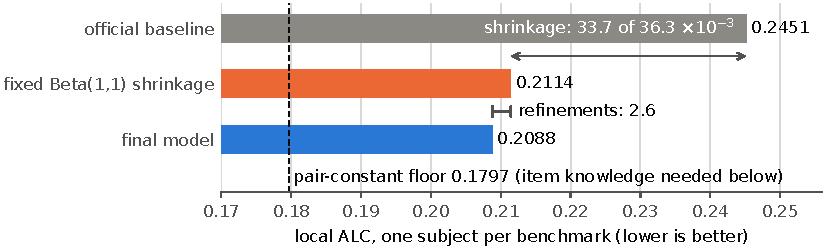
\includegraphics[width=0.9\linewidth]{fig_teaser.pdf}\\[6pt]
\raggedright
\textbf{Local, leave-one-benchmark-out} (4 held-out benchmarks, one subject per benchmark, 10 seeds, paired):
\begin{itemize}
\item Official baseline (empirical mean) \textbf{0.2451} $\to$ fixed Beta(1,1) shrinkage \textbf{0.2114} $\to$
  final model \textbf{0.2088}.
\item Shrinkage is Laplace's rule, $(s+1)/(n+2)$: \emph{nothing is fitted}.
\item The refinements add $2.6\ee{3}$, concentrated at budgets 7--31; their $t$-interval over fold means,
  $[-6.3,+1.1]\ee{3}$, includes zero.
\end{itemize}
\end{tcolorbox}

\begin{tcolorbox}[block, title={Result 2: 89 unseen benchmarks, pre-registered}]
Frozen archives, no refit, 2{,}610 pairs, 89 public benchmarks never used for fitting.
\begin{center}\fontsize{21}{26}\selectfont
\begin{tabular}{@{}lll@{}}
\toprule
comparison & $\Delta$ALC$\times10^{3}$ [95\% CI] & reading\\
\midrule
shrinkage $-$ official baseline & $-32.7$ \;$[-37.1,-28.2]$ & \textbf{confirmed} (82 of 89)\\
final model $-$ shrinkage & $+0.2$ \;$[-0.9,+1.5]$ & no difference detected\\
\bottomrule
\end{tabular}\end{center}
The primary outcome is \textbf{inconclusive} at the pre-registered $\pm1\ee{3}$ minimum effect, so the hierarchical
refinements are \textbf{unproven}. These benchmarks had been used earlier for a simulator check (disclosed in the
pre-registration).
\end{tcolorbox}

\begin{tcolorbox}[block, title={The model (pure Python + NumPy, 5\,KB zipped)}]
Motivated by $\operatorname{logit}P(y{=}1)=\mu_b+\theta_{sb}-\beta_i+\gamma_{g(i)}$, but computed in stages:
\begin{enumerate}
\item \textbf{Pair level (always).} $\mu_b\sim t_3(G/2,s)$, a \emph{hedged} centre halfway between the pooled level
  and 50\% (cuts worst-case regret on easy benchmarks by 29--50\%); $\theta_j\sim\mathcal N(0,\tau^2)$;
  posterior mean $q_0$ for the target pair.
\item \textbf{Same-key branch.} If any subject has a label on an item with the same content key, mix in a shared
  item difficulty, weighted by the posterior probability that the key denotes one item.
\item \textbf{Item-group branch.} Else, offsets for \texttt{item\_features} cells from the subject's own labels.
\item \textbf{Otherwise} (every budget-0 prediction) output $q_0$; clip to $[0.005,0.995]$.
\end{enumerate}
Labels are acquired at random: four smarter policies gained at most $0.27\ee{3}$, as expected when the predictor
cannot tell unlabelled items apart.
\end{tcolorbox}

\begin{tcolorbox}[block, title={Limitations and reproduction}]
\begin{itemize}
\item Four local held-out benchmarks; the refinements' benefit is not established at benchmark level.
\item Floor, ceiling and oracle figures are in-sample; runtime LLM priors were not tested.
\item \textbf{Three reproduction tiers}: saved-result checks from a clone (\texttt{--quick}; rows needing gated data
  or feedback SKIP); live reruns from public data (including the 89-benchmark check); checks that need our formative
  feedback (not released).
\end{itemize}
{\fontsize{19}{23}\selectfont\color{muted} Code (MIT): github.com/Shashwat-srivastav/s2wish-paiec2026, tag
\texttt{v1.1-camera-ready}. Final archive SHA-256 \texttt{a4b0e841\ldots92685b86}. Code and text were developed
with Claude Code (Anthropic); the author checked every claim and number.\par}
\end{tcolorbox}

\end{minipage}\hfill
\begin{minipage}[t]{0.488\linewidth}\vspace{0pt}

\begin{tcolorbox}[block, title={Result 3: what is left, and what could close it}]
\textbf{Pair-constant floor.} A rule predicting one value per pair and budget scores at least $a(1-a)$ on every
pair, where $a$ is the pair's accuracy (Proposition 4).
\begin{itemize}
\item Locally the floor is \textbf{0.1797} against \textbf{0.2088} for the final model: a gap of $0.0291$.
\ifplatformstats
\item On our saved platform draws, the largest gain any pair-constant rule could give is $0.0218$ ALC
  (95\% CI up to $0.033$; in-sample, 26 pair-slots from three model versions).
\fi
\item Below the floor, only \textbf{item-varying} predictions help.
\end{itemize}
\textbf{Item oracle} (in-sample): adding true Rasch item effects to the model's own pair-level prediction closes
\textbf{about half} of the closable budget-0 gap (0.48; 0.45 leave-pair-out).\\[8pt]
\begin{minipage}[t]{0.52\linewidth}\vspace{0pt}
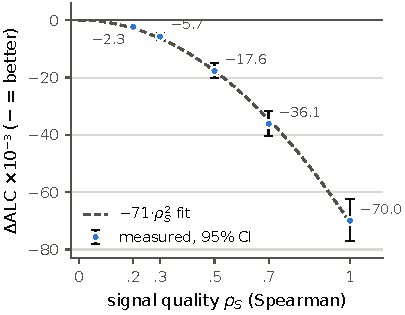
\includegraphics[width=\linewidth]{fig_rho_value.pdf}
\end{minipage}\hfill
\begin{minipage}[t]{0.45\linewidth}\vspace{0pt}
\textbf{Value of a label-free difficulty signal} grows roughly with $\rho_S^2$ (synthetic signal: true difficulty
plus noise):
\begin{itemize}
\item $\rho_S=0.3$: worth $5.7\ee{3}$
\item $\rho_S\approx0.5$: worth $0.018$
\item without shrinkage it \emph{hurts} below $\rho_S\approx0.5$
\end{itemize}
Our offline LLM rating reached $\rho_S=0.19$--$0.34$; a \textbf{runtime LLM item prior} is the most promising
untested direction.
\end{minipage}
\end{tcolorbox}

\begin{tcolorbox}[block, title={Reading per-pair feedback}]
At budget 0 the model predicts one constant $p_0$ per pair, so the reported budget-0 Brier score gives the pair's
accuracy:
\[ B_0=a(1-p_0)^2+(1-a)p_0^2 \quad\Longrightarrow\quad a=\frac{B_0-p_0^2}{1-2p_0}. \]
\vspace{-12pt}
\begin{itemize}
\item \textbf{Error bound} from six-decimal rounding: $\varepsilon(p_0)=\eta/|1-2p_0|+\eta$, $\eta=5\ee{7}$.
\item \textbf{Reflection pitfall:} without the archive's own $p_0$, only $a(1-a)$ is identified, and a wrong $p_0$
  flips every accuracy.
\item \textbf{Conditional replays:} if predictions depend only on the count of revealed successes (assumption A4),
  any pair-constant rule can be replayed in-sample without uploading it.
\end{itemize}
\ifplatformstats
\begin{minipage}[t]{0.50\linewidth}\vspace{0pt}
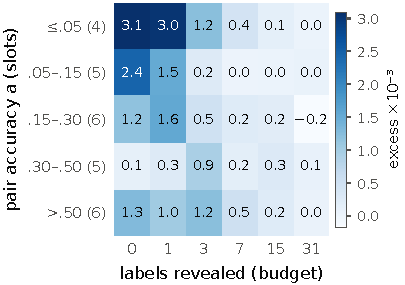
\includegraphics[width=\linewidth]{fig_excess_map.pdf}
\end{minipage}\hfill
\begin{minipage}[t]{0.47\linewidth}\vspace{0pt}
Of the loss above $a(1-a)$ that more labels could remove, \textbf{71\%} sits at budgets 0--1 and \textbf{56\%} on
pairs with accuracy $\le0.15$ (conditional replay, our own feedback only, no ID named).
\end{minipage}
\fi
\end{tcolorbox}

\begin{tcolorbox}[block, title={What did not work (60 logged experiments, 22 pre-registered)}]
\resizebox{\linewidth}{!}{%
\begin{tabular}{@{}lll@{}}
\toprule
component & $\Delta$ALC$\times10^3$ vs final [95\% CI] & decision\\
\midrule
lexical residual smoothing & $+1.68$ $[+1.08,+2.30]$ & dropped: worse\\
gp-IRT (our reimplementation) & $+6.88$ $[+4.80,+8.94]$ & not promoted\\
re-tuned shrinkage strength & $+0.74$ $[-0.28,+1.85]$ & no change\\
fitted temperature & $+0.40$ $[+0.24,+0.56]$ & already calibrated\\
symmetric mixture prior & $+0.52$ $[+0.22,+0.80]$ & retired: worse\\
robust / metadata / name priors & best gain $\le1.0$ & below the gate\\
smarter acquisition (4 policies) & best gain $\le0.27$ & random kept\\
\bottomrule
\end{tabular}}\\[6pt]
One to three labels cannot tell prior centres a third of a logit apart, and ability is mostly benchmark-specific.
\end{tcolorbox}



\end{minipage}

\end{document}
